\documentclass[12pt]{article}

\usepackage[utf8]{inputenc}
\usepackage{latexsym,amsfonts,amssymb,amsthm,amsmath}
\usepackage{float}

\setlength{\parindent}{0in}
\setlength{\oddsidemargin}{0in}
\setlength{\textwidth}{6.5in}
\setlength{\textheight}{8.8in}
\setlength{\topmargin}{0in}
\setlength{\headheight}{18pt}
\usepackage{graphicx}
\usepackage{tikz}

\usepackage{hyperref}
\hypersetup{
    colorlinks=true,
    linkcolor=blue,
    filecolor=magenta,      
    urlcolor=cyan,
    pdftitle={Overleaf Example},
    pdfpagemode=FullScreen,
}

\urlstyle{same}

\usepackage{caption}
\DeclareCaptionFormat{citation}{%
  \ifx\captioncitation\relax\relax\else
    \captioncitation\par
  \fi
  #1#2#3\par}
\newcommand*\setcaptioncitation[1]{\def\captioncitation{\textit{Source:}~#1}}
\let\captioncitation\relax
\captionsetup{format=citation,justification=centering}


\title{MATH1034OL1 Pre-Calculus Mathematics Sections Final Review and Cheatsheet for Calculus}
\author{Elijah Renner}

\begin{document}

\maketitle

\vspace{0.5in}

\tableofcontents

\section{About}

Here's all the information you need for the midterm. \\

\section{Content Before Midterm}

In order to avoid redundancy, only content from after the midterm will be included. See the the midterm review for content before the review: \url{https://tamath.org/media/precalculus/7.17/7.17.pdf}.\\

\section{Inverse Trigonometric Functions}

The three inverse trigonometric functions are \(\arccos\), \(\arcsin\), and \(\arctan\). These functions have the property\\

\[\arccos(x)=A\]
\[\cos(A)=x\]\\

In other words, \(\cos\) and \(\arccos\) are inverses of each other. They're helpful for determining an angle given its \(\sin, \cos,\) or \(\tan\) value.\\

When we're finding \(\arcsin(x)\), we restrict the range of \(\arcsin\) such that it remains a function (that is, there are no two outputs \(\arcsin(x)\) for one input \(x\)). We do this for all inverse trigonometric functions. Here are the restrictions:\\

\begin{figure}[H]
	\centering
	\includegraphics[scale=0.6]{arcf.gif}
	\caption{Credit: \url{https://www.mathnstuff.com/math/spoken/here/2class/330/arc.htm}}
\end{figure}

Problem: Find the Exact value of \(\sec\{\arctan[\sin(\arccos(\frac{-1}{2}))]\}\).\\

First, recall that \(\arccos(\frac{-1}{2})\) will be the angle whose cosine value is \(\frac{-1}{2}\). We know this angle is \(\frac{2\pi}{3}\) using the rules above.\\

Next, we determine that \(\sin(\frac{2\pi}{3})=\frac{\sqrt{3}}{2}\). This is where things get a little more complicated. \(\arctan(\frac{\sqrt{3}}{2})\) isn't an angle with reference angle \(30^{\circ}, 45^{\circ}, 60^{\circ}, 90^{\circ}\). This is fine because, when we zoom out, we're asked to find \(\sec(\arctan(\frac{\sqrt{3}}{2}))\). We know that the triangle formed by the angle \(\arctan(\frac{\sqrt{3}}{2})\) has \(\text{opp}=\sqrt{3}\) and \(\text{adj}=2\). We use the pythagorean theorem to find the hypotenuse:\\

\[(\sqrt{3})^2+2^2=c^2\]
\[\implies c=\sqrt{3+4}=\sqrt{7}\]\\

Hence, \(\text{hyp}=\sqrt{7}\). Even though the angle \(\arctan(\frac{\sqrt{3}}{2})\) doesn't form a special triangle, we can still find its \(\sec\) value using the sides of the triangle it forms:\\

\[\sec\left(\arctan\left(\frac{\sqrt{3}}{2}\right)\right)=\frac{\text{hyp}}{\text{adj}}=\frac{\sqrt{7}}{2}\]\\

Knowing this, \(\sec\{\arctan[\sin(\arccos(\frac{-1}{2}))]\}=\frac{\sqrt{7}}{2}\).

\section{Polynomial Long Division}

Polynomial division isn't easily explained in notes, but it's very important!. Here is my recommended resource for polynomial division:\\

\url{https://www.mathsisfun.com/algebra/polynomials-division-long.html}

\section{Remainder Theroem}

\begin{figure}[H]
	\centering
	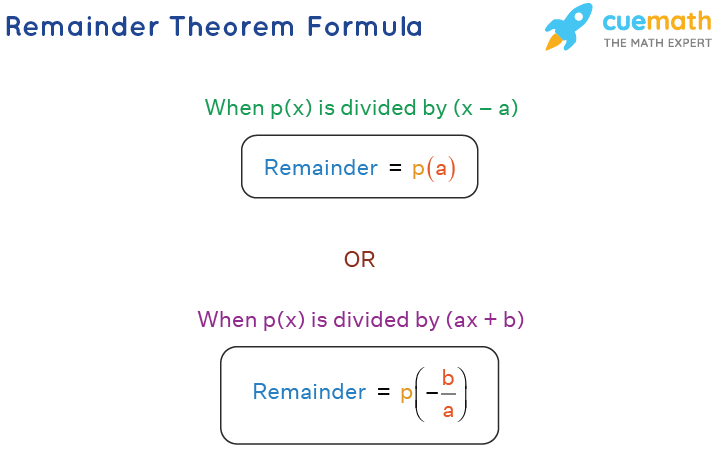
\includegraphics[scale=0.6]{rt.png}
	\caption{Credit: \url{https://www.cuemath.com/algebra/remainder-theorem/}}
\end{figure}


\section{Descarte's Rule of Signs}

\begin{figure}[H]
	\centering
	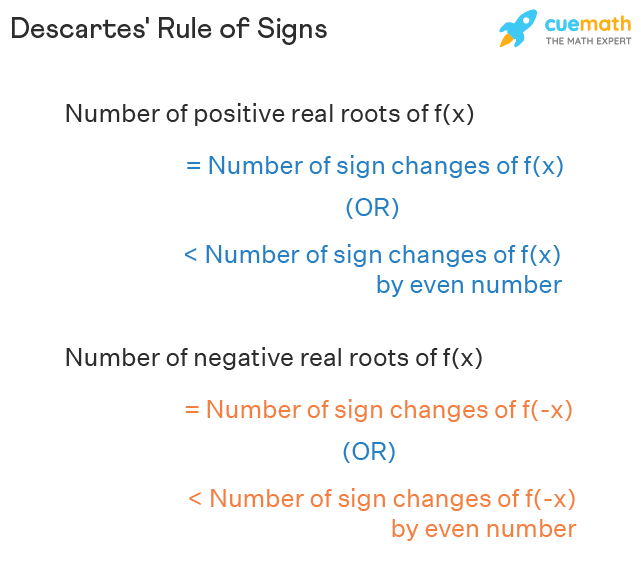
\includegraphics[scale=0.6]{drs.png}
	\caption{Credit: \url{https://www.cuemath.com/algebra/descartes-rule-of-signs/}}
\end{figure}

\begin{figure}[H]
	\centering
	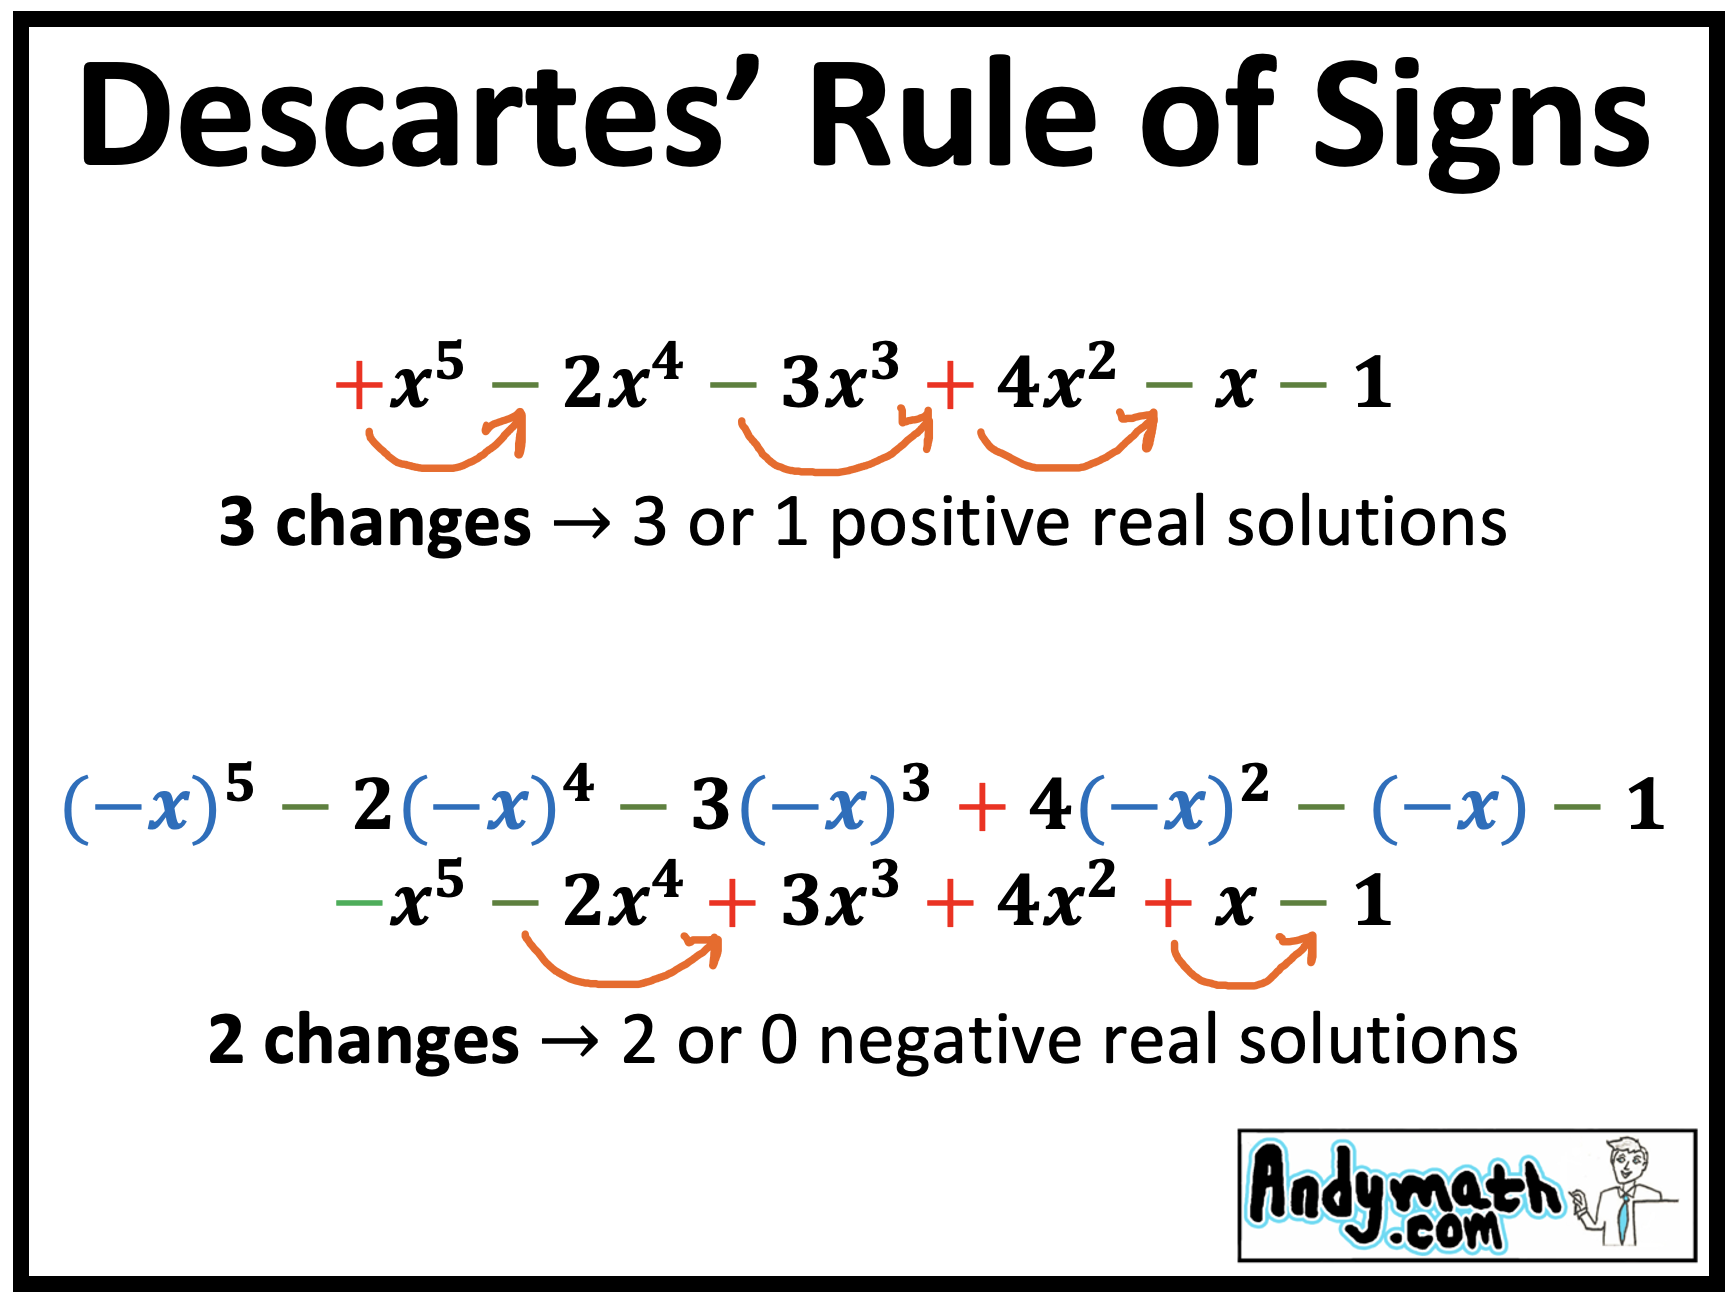
\includegraphics[scale=0.3]{drs2.png}
	\caption{Credit: \url{https://andymath.com/descartes-rule-of-signs/}}
\end{figure}

\section{Factors of Polynomials}

If a polynomial has a zero of \(x=a\) whose multiplicity is \(b\), \((x-a)^b\) is a factor.

\section{Included Angles}

\begin{figure}[H]
	\centering
	\includegraphics[scale=1]{included.gif}
	\caption{Credit: \url{https://www.mathopenref.com/angleincluded.html}}
\end{figure}

\section{Law of Cosines}

We use the law of cosines to "solve" (find all angles and sides) of a triangle when we are given either a) three sides or b) two sides and the included angle.\\

Consider the triangle\\

\begin{figure}[H]
	\centering
	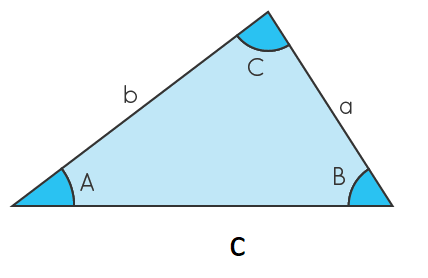
\includegraphics[scale=0.6]{abc.png}
	\caption{Credit: \url{https://www.cuemath.com/questions/for-triangle-abc-with-sides-a-b-and-c-the-law-of-cosines-states-the-following/}}
\end{figure}

with sides \(a\), \(b\), and \(c\) and angles \(A\), \(B\), and \(C\). We define the law\\

\[a^2=b^2+c^2-2bc\cos A\]

which can be rewritten by swapping any two of the variables:\\

\[b^2=a^2+c^2-2ac\cos B\]
\[c^2=a^2+b^2-2ab\cos C\]

These can also be rewritten algebraically to solve for angles \(A\), \(B\), or \(C\).

\section{Law of Sines}

The law of sines relates the proportions of sides to the sine values of the angles opposite the sides:\\

\[\frac{a}{\sin A}=\frac{b}{\sin B}=\frac{c}{\sin C}\]

The rule is useful when we are given either a) two angles and one side, or b) two sides and a non-included angle.\\

\section{Complex and Imaginary Numbers}

Let \(z\) be the complex number \(a+bi\). The conjugate of \(z\) is \(\bar{z}=a-bi\). One useful property to remember is that \(z\bar{z}\) is a real number.

\section{Asymptotes and x-Intercepts of Rational Functions}

\begin{figure}[H]
	\centering
	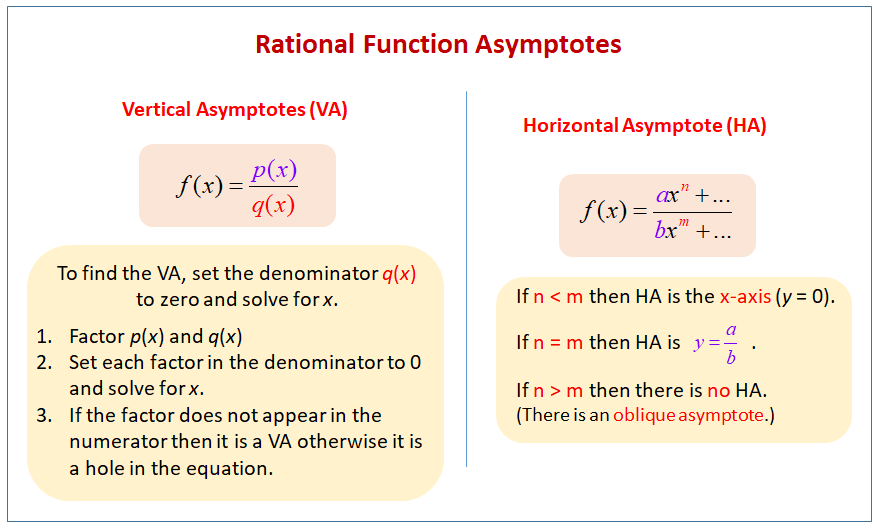
\includegraphics[scale=.75]{rational.png}
	\caption{Credit: \url{https://www.onlinemathlearning.com/rational-functions.html}}
\end{figure}

The x-intercepts of a rational function are the values that make the numerator equal to zero.\\

If the degree of the top polynomial is one greater than the bottom polynomial, there exists an oblique or slant asymptote:\\

\begin{figure}[H]
	\centering
	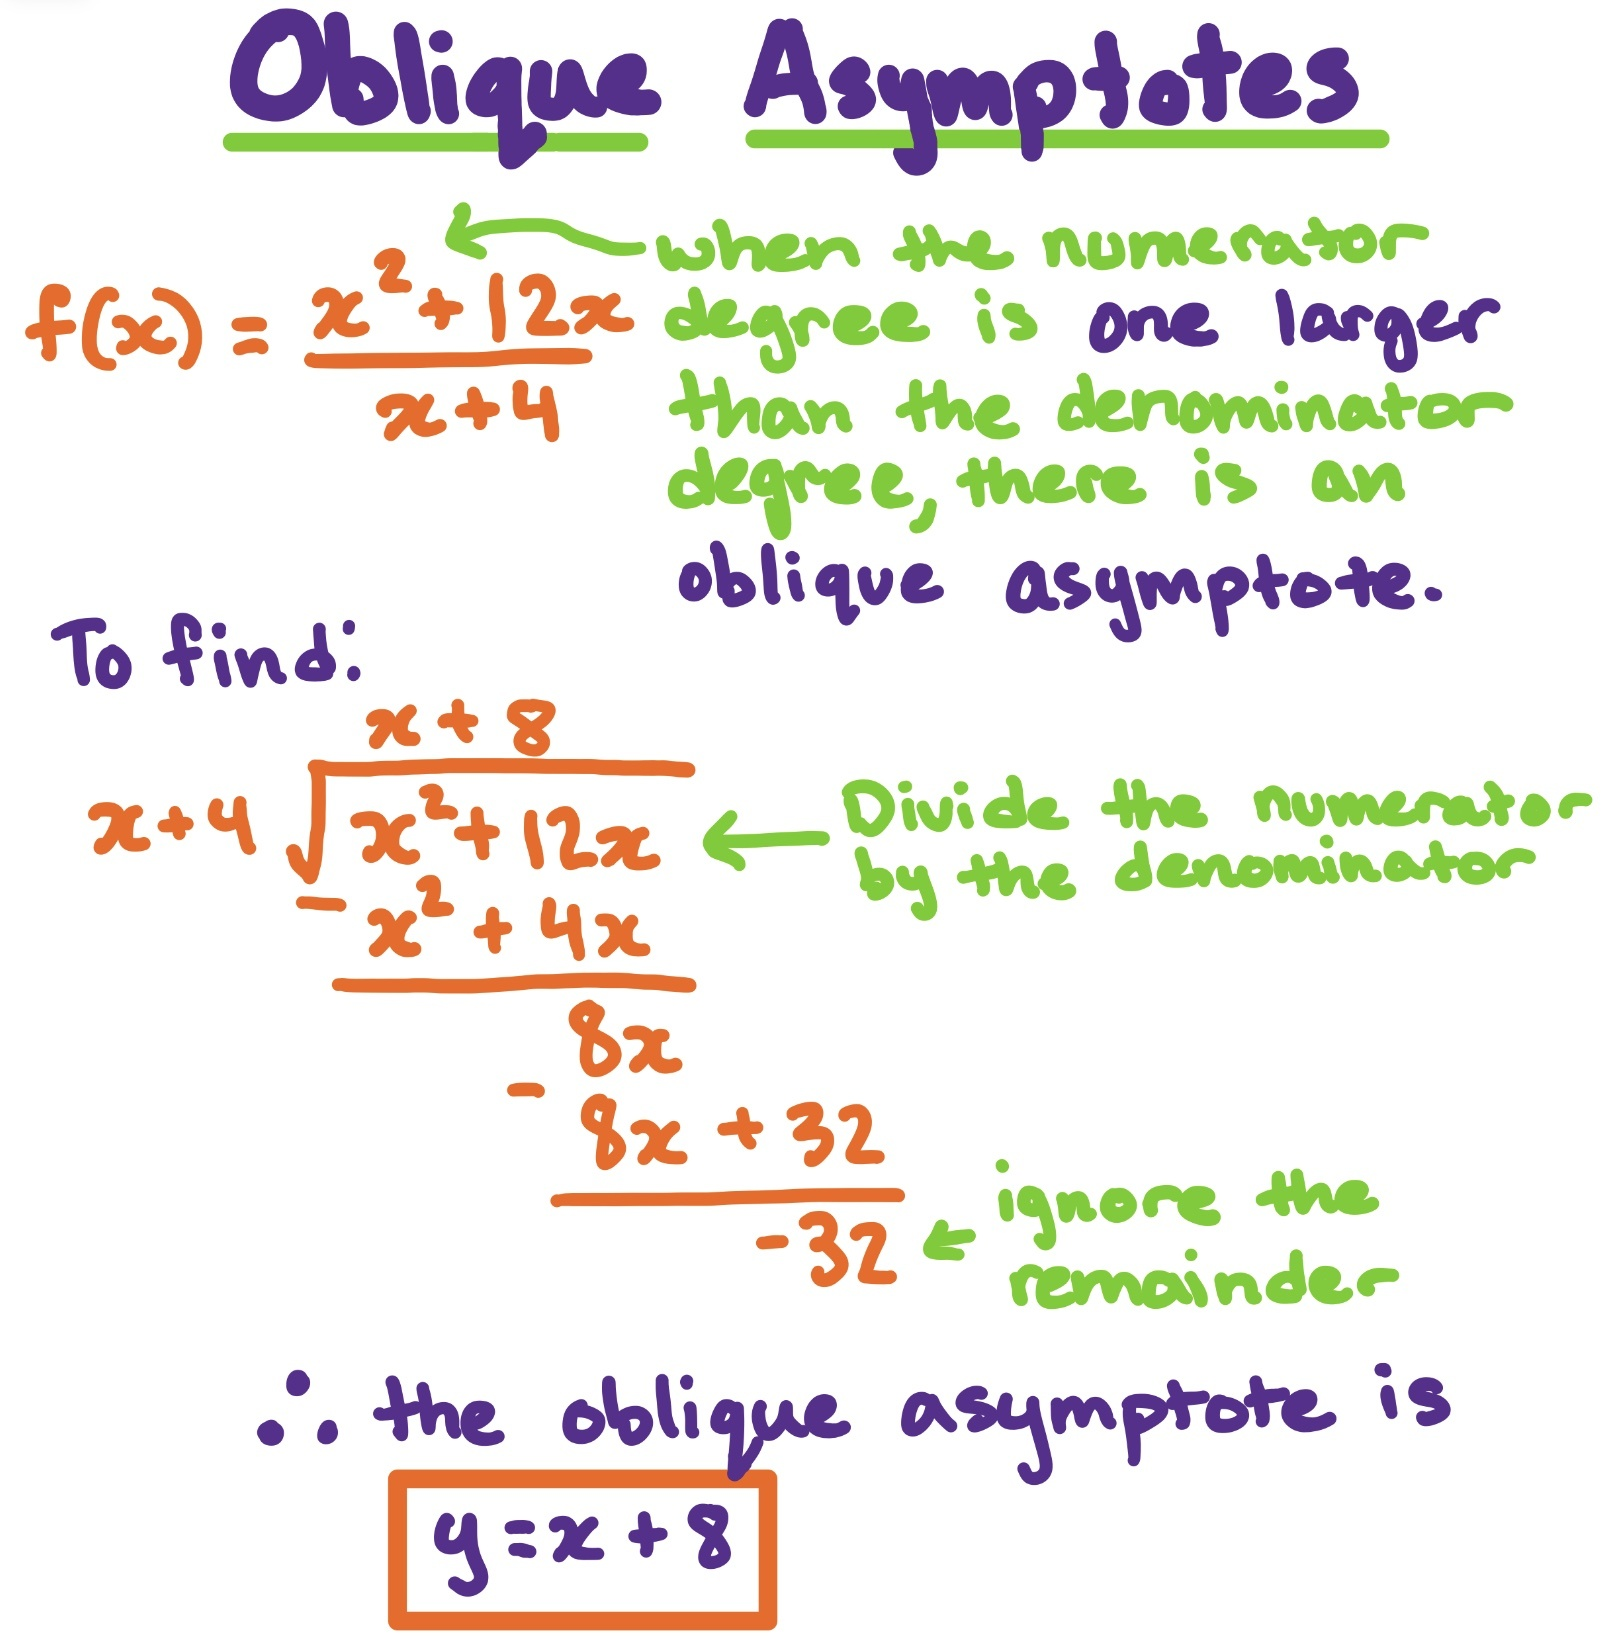
\includegraphics[scale=.2]{oblique.jpg}
	\caption{Credit: \url{https://www.expii.com/t/oblique-asymptotes-of-rational-functions-5138}}
\end{figure}

Some final notes about asymptotes:\\

Horizontal asymptotes and oblique asymptotes may be crossed by the rational function, but vertical asymptotes may not (because they're the values where the function is undefined).\\

To determine if some asymptote intersects a rational function, set them equal and look for a contradiction. If there isn't a contradiction, the rational function intercepts that asymptote at the value of x in that equality.\\

\section{Compound Interest and the Natural Base}

For an initial amount \(P\), interest rate \(r\), compounding rate per time period \(t\), and time periods elapsed \(t\), we define the final amount \(A\) as\\

\[A=P\left(1+\frac{r}{n}\right)^{nt}\]\

If the compounding is continuous, meaning it's calculate infinitely many times in a given compounding period, the base is \(e\approx2.718\). Let's derive \(e\):\\

\[e=\lim_{x\to \infty}\left(1+\frac{1}{n}\right)^{1\cdot n}\]\

Hence, to calculate the new amount given an initial amount \(P\) after \(t\) time periods with interest rate \(r\), we use \(A=Pe^{rt}\)\\

For \(P=1000\), \(t=3\), and \(r=13\%\): \(A=1000e^{0.13\cdot 3}\approx1,476.98\)\\

\section{Logarithms}

\begin{figure}[H]
	\centering
	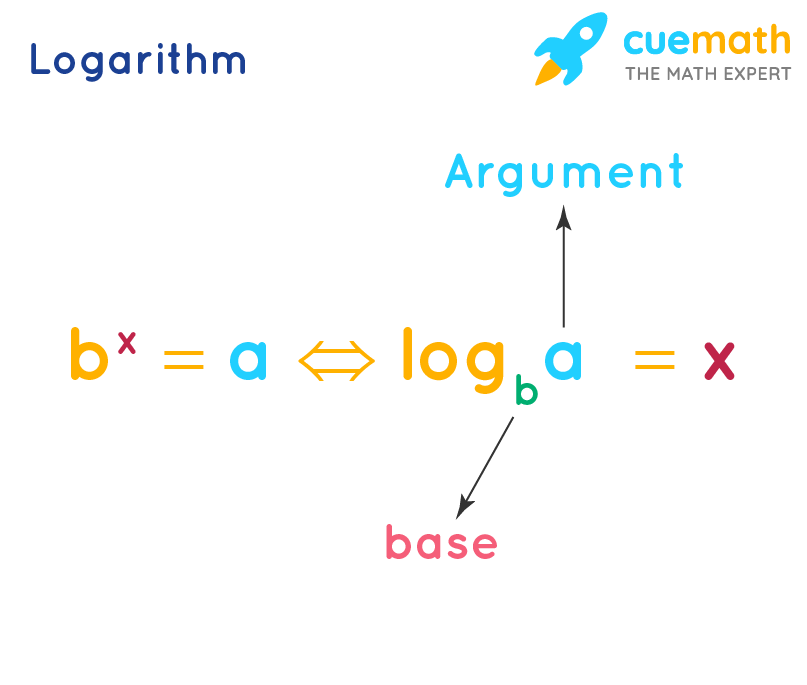
\includegraphics[scale=0.6]{logs.png}
	\caption{Credit: \url{https://www.cuemath.com/log-formulas/}}
\end{figure}

In plain language: the value of a logarithm is the power the base must be raised to in order to get the argument.\\

Logarithms are also the inverses of exponential functions. This means that for \(f(x)=b^x\), \(f^{-1}(x)=\log_bx\). Given this property, we know that a an exponential function and its corresponding inverse logarithmic function will reflect over the line \(y=x\):\\

\begin{figure}[H]
	\centering
	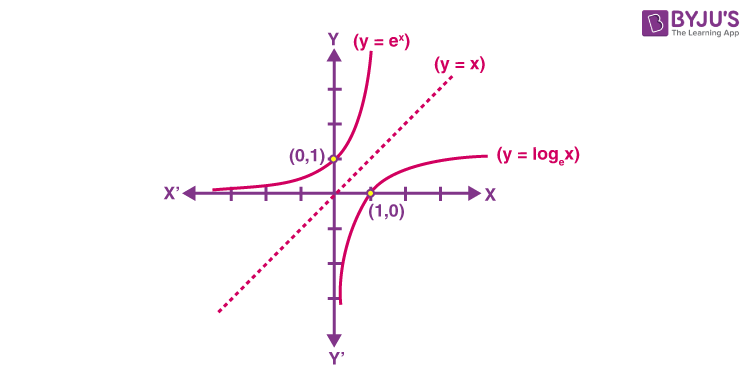
\includegraphics[scale=0.5]{inv.png}
	\caption{Credit: \url{https://byjus.com/maths/exponential-and-logarithmic-functions/}}
\end{figure}

Here are the rules to find the inverse of a logarithmic or exponential function:\\

\begin{figure}[H]
	\centering
	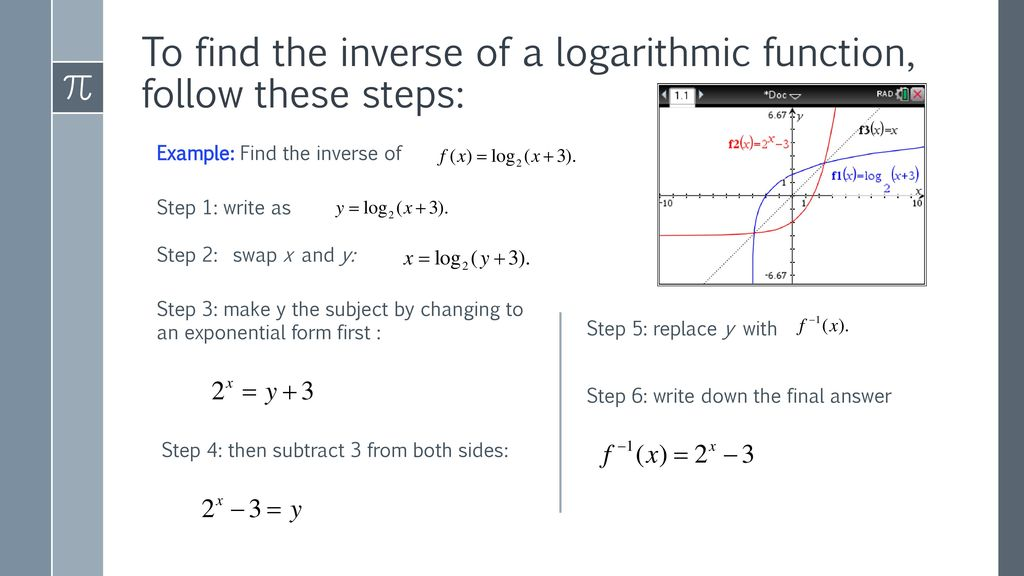
\includegraphics[scale=1.75]{loginv.jpg}
	\caption{Credit: \url{https://slideplayer.com/slide/12938368/}}
\end{figure}

\begin{figure}[H]
	\centering
	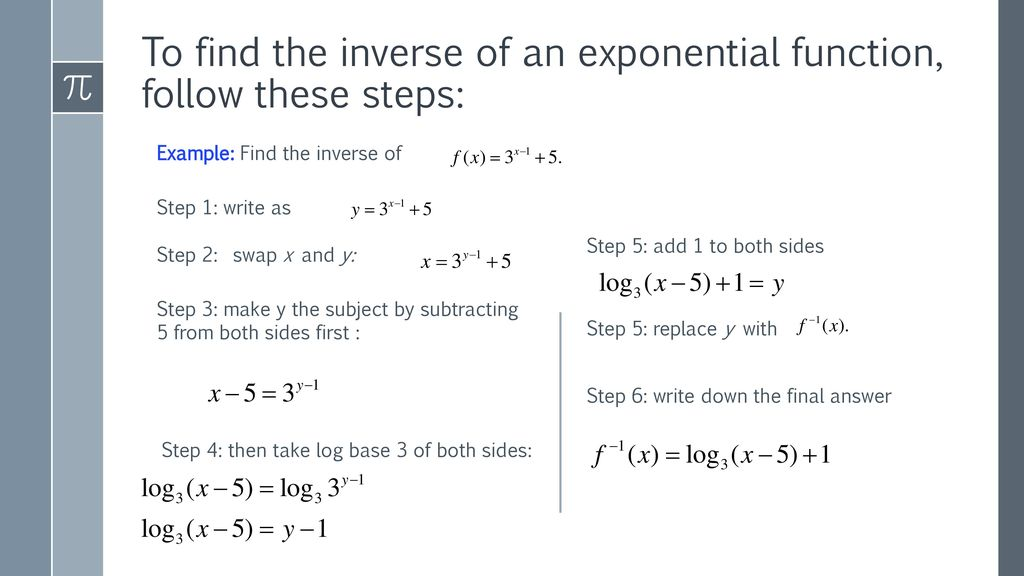
\includegraphics[scale=1.75]{expinv.jpg}
	\caption{Credit: \url{https://slideplayer.com/slide/12938368/}}
\end{figure}


We didn't discuss logarithmic graphs in class, but here are some important properties to understand:\\

\begin{figure}[H]
	\centering
	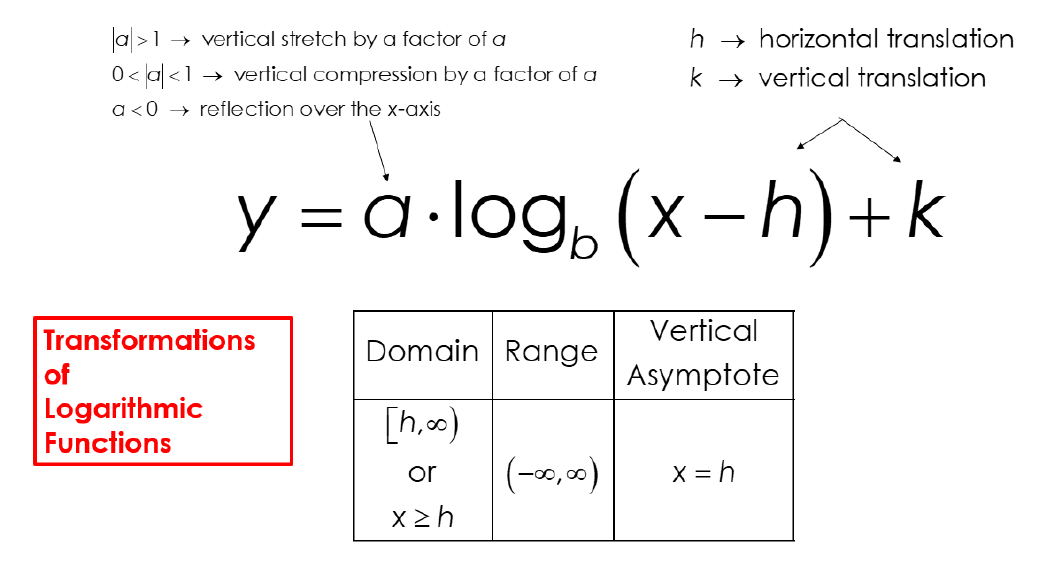
\includegraphics[scale=.45]{loggraph.png}
	\caption{Credit: \url{https://goodsifyet.shop/product_details/7113278.html}}
\end{figure}

There exists an asymptote at \(x=h\) because logarithmic functions may not have an argument less than 0. Similarly, they also may not have a negative base.\\

There are some rules for logarithms, too:\\

\begin{figure}[H]
	\centering
	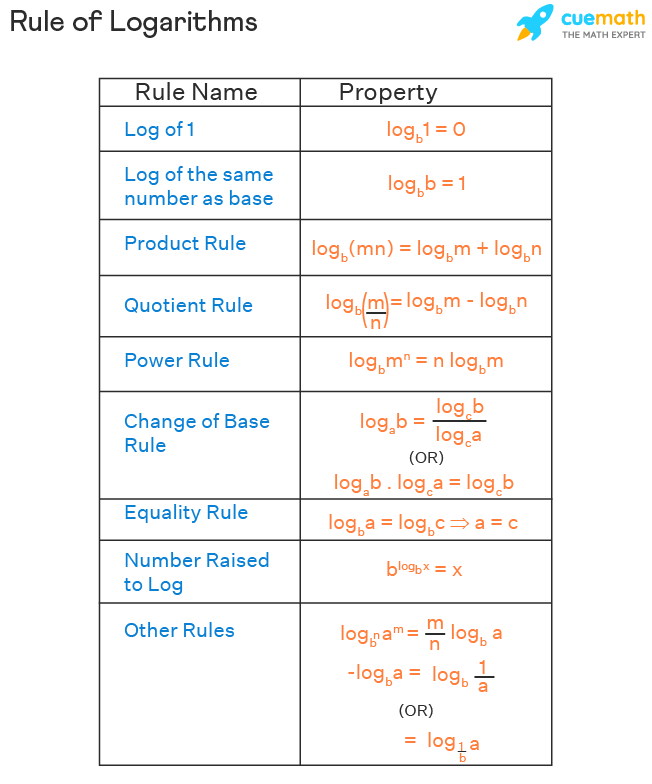
\includegraphics[scale=.52]{logrules.png}
	\caption{Credit: \url{https://www.cuemath.com/algebra/log-rules/}}
\end{figure}

\section{Fraction Exponents}

\[x^{\frac{a}{b}}=\sqrt[\leftroot{-2}\uproot{2}b]{x^a}=\left(\sqrt[\leftroot{-2}\uproot{2}b]{x}\right)^a\]

\section{Exponential Growth and Decay with the Natural Base}

Today's class only introduced the idea of exponential growth and decay, so I'll cover that here.\\

We define the general equation for exponential growth as\\

\[y(t)=ae^{kt}\]\\

where \(y(t)\) is the value at time \(t\), \(a\) is the initial value, and \(k\) is the growth constant.\\

Usually, we'll need to solve for \(k\) given information.\\

Problem: when will a population reach 50000 people if there are 10000 people initially and triples every two years?\\

Since the questions gives us the growth rate ("triples every two years"), we'll create the datapoint (2,30000) which repreesnts the population after two years.\\ 

We'll then plug this and given information into our equation \(y(t)=ae^{kt}\) and solve for \(k\), the growth constant:\\

\[30000=10000e^{2k}\]
\[\implies 3=e^{2k}\]
\[\implies \ln 3=\ln e^{2k}=2k\]
\[\implies k=\frac{\ln 3}{2}\]\\

Now we can write the population as an exponential function of time:\\

\[y(t)=10000e^{kt}=10000e^{\frac{\ln 3}{2}t}\]\\

The question asks for the time when the population \(y(t)\) is 50000, so we plug that in:\\

\[50000=10000e^{\frac{\ln 3}{2}t}\]
\[\implies 5=e^{\frac{\ln 3}{2}t}\]
\[\implies \ln 5=\ln e^{\frac{\ln 3}{2}t}=\frac{\ln 3}{2}t}\]
\[\implies t=\frac{\ln 5}{\left(\frac{\ln 3}{2}\right)}=\frac{2\ln 5}{\ln 3}}\text{ years}\]\\

Also, \(e\) is the base since it's easily differentiable in calculus. I had to look this up because I was confused why we didn't use simple bases (like \(\frac{1}{2}\)) for half-life decay.\\


\end{document}
